\newpage
\section{Test Results} \label{sec:apptestres}

\subsection{Test 28: Pump Operations}
\label{sec:test28result}

The pump was connected via crocodile connections to a power supply set to 24 V. The power supply was then switched on and the current was read off. This set-up can be seen in Figure \ref{fig:pump-testing}.

It was found that when the power supply was switched on the current went up to 600 mA for less than one second. It then settled to 250 mA. By covering the air intake, simulating air intake from a lower pressure, the current drops to 200 mA. By covering the air output, simulating pushing air into a higher pressure, the current rises to 400 mA.

Therefore the power for each of these conditions is 14.4 W at turn on, 6 W in normal use, 4.8 W when sucking from low pressure, 9.6 W when pushing to high pressure.


\begin{figure}[H]
    \begin{align*}
        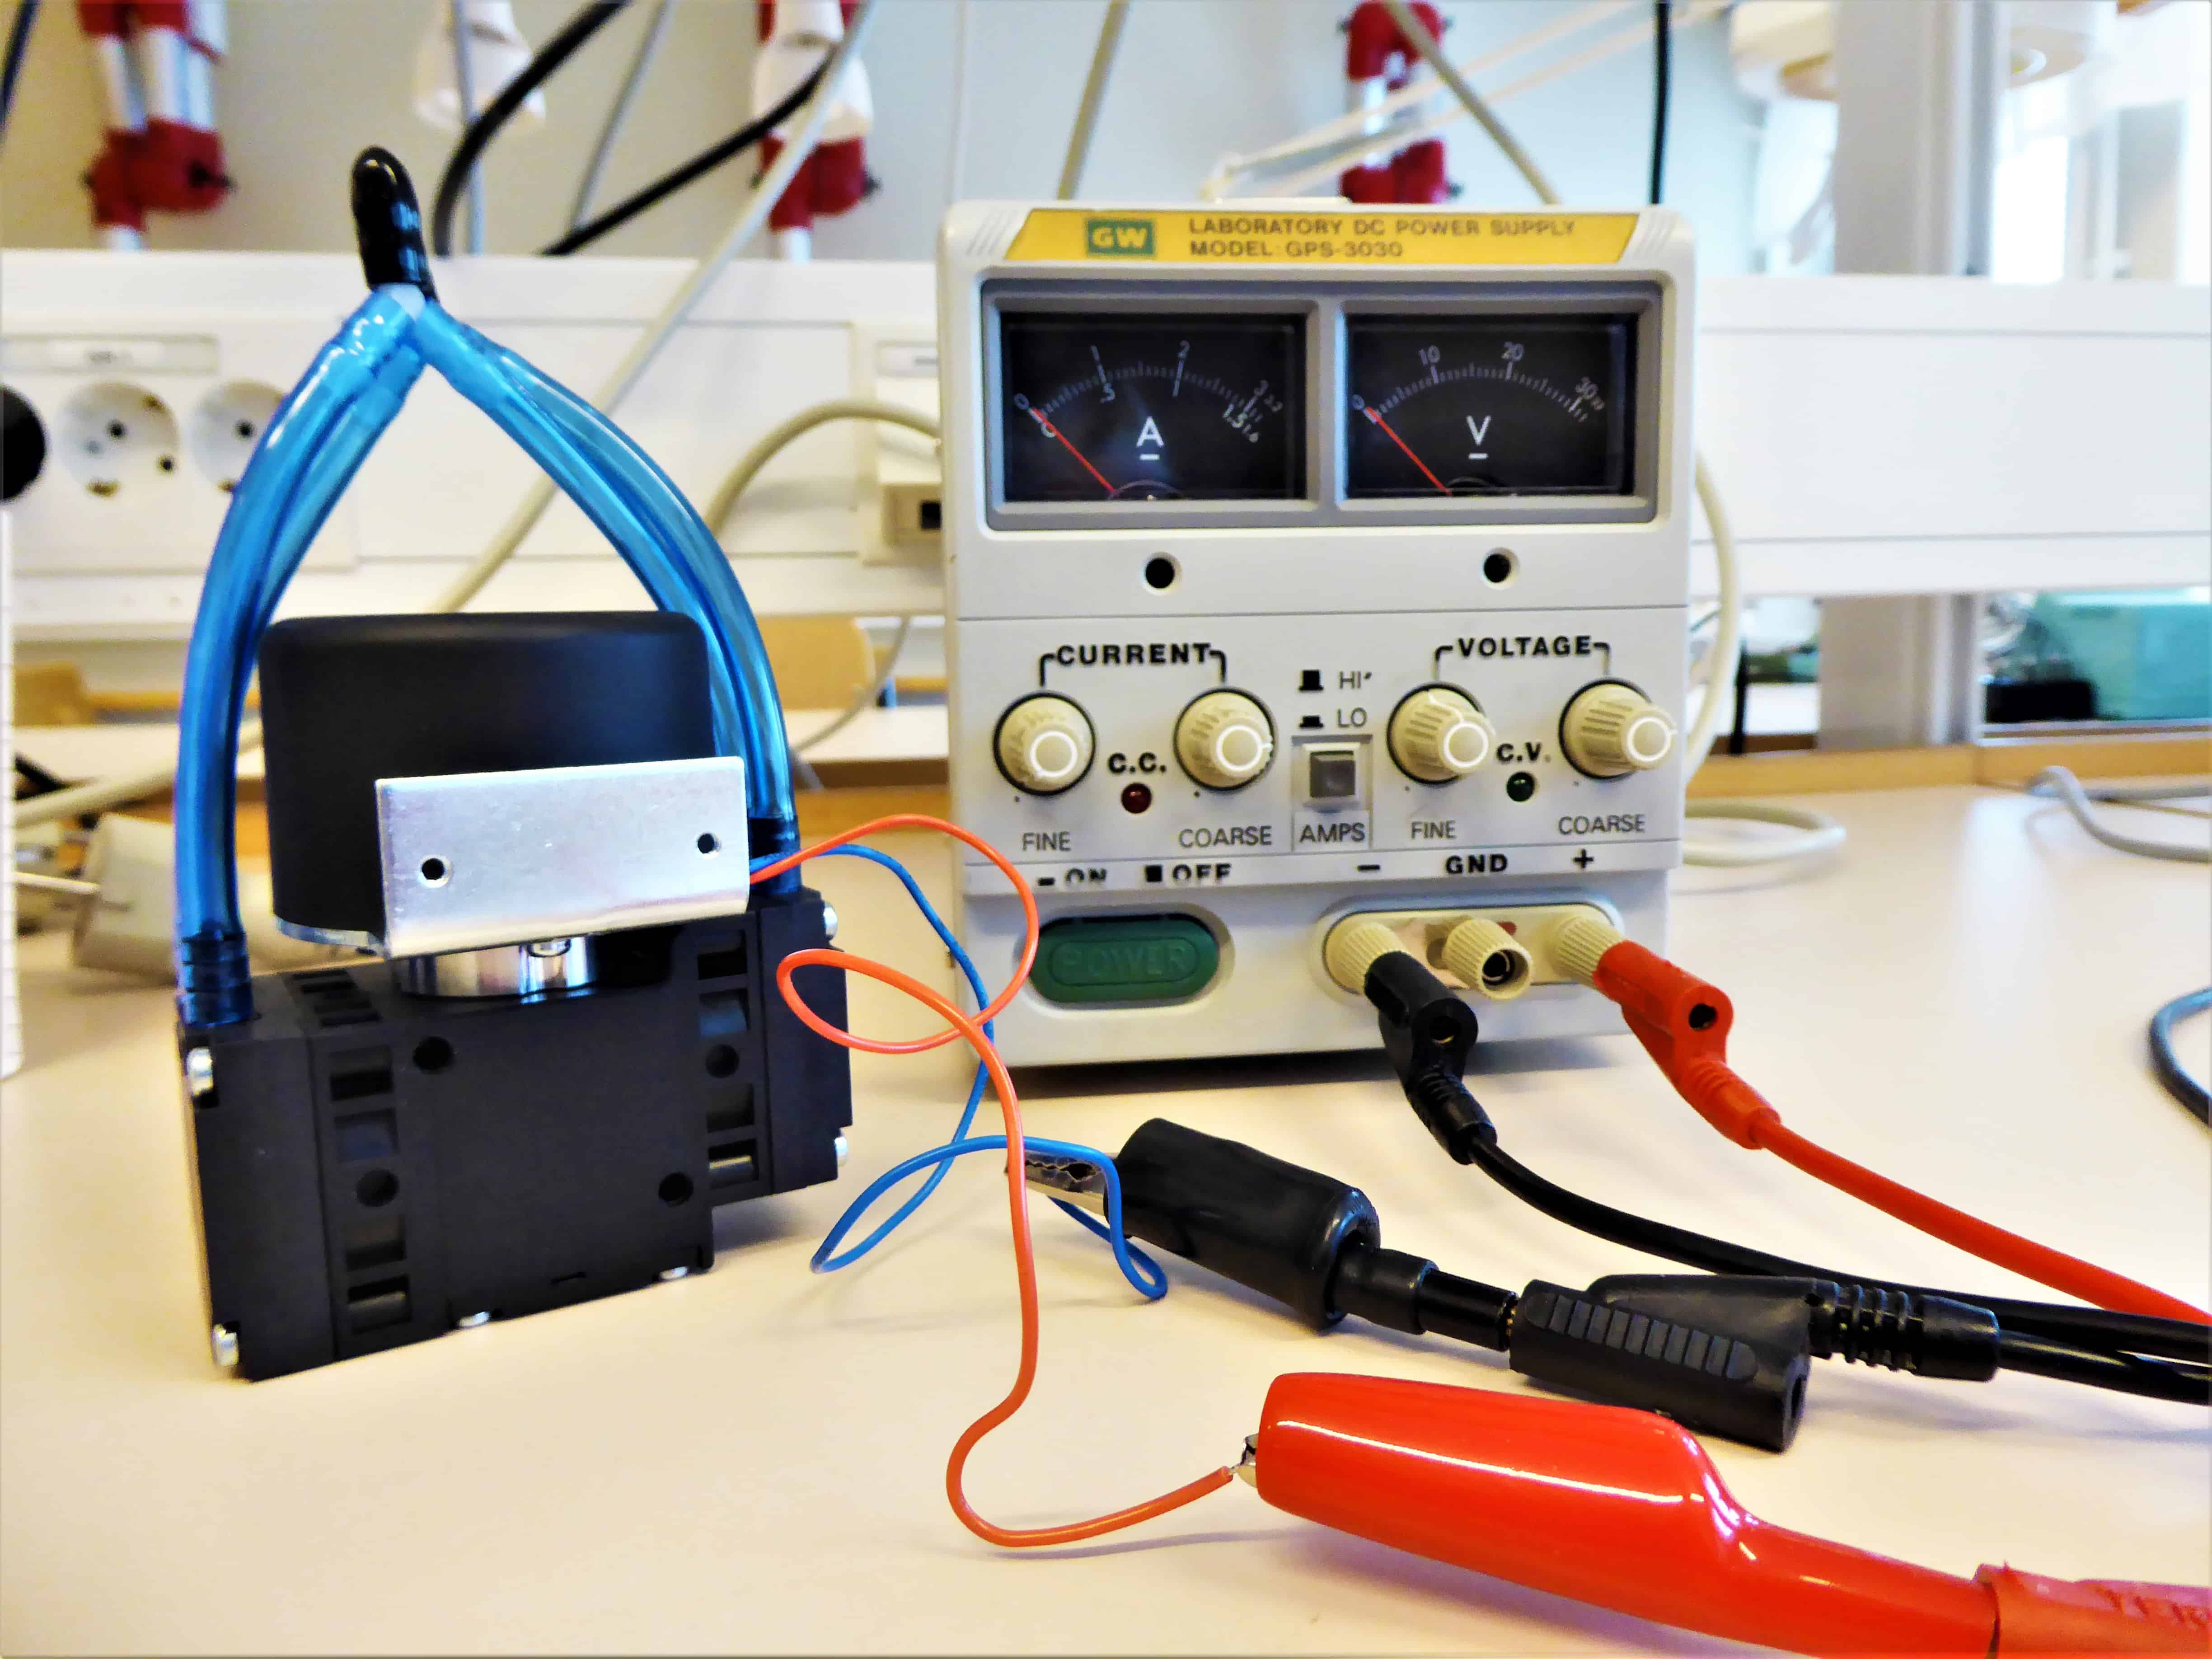
\includegraphics[width=1\linewidth]{5-experiment-verification-and-testing/img/pump-testing.png}
    \end{align*}
    \caption{Photo Showing the Set-up for the Pump Testing in the Laboratory.} \label{fig:pump-testing}
\end{figure}

\subsection{Test 18: Pump Low Pressure}\label{subsection:pumplowpressuretest}

The pump was tested at low pressure using a small vacuum chamber that is capable of going down to \SI{1}{\hecto\pascal}. For this test the chamber was only taken down to \SI{30}{\hecto\pascal} as this is the expected pressure at 24 km, the highest altitude that will be sampled. The experiment set-up can be seen in Figure \ref{fig:pump-low-pressure-set-up}. The pump was connected to the power supply via two cables. It was also screwed into the base plate to prevent it from moving due to its own vibration during the test. A vacuum pump was connected to the chamber wall with a pressure sensor attached to monitor the pressure inside the chamber. 

\begin{figure}[H]
    \begin{align*}
        \includegraphics[width=1\linewidth]{5-experiment-verification-and-testing/img/low-pressure-set-up.png}
    \end{align*}
    \caption {Photo Showing the Set-up of the Vacuum Chamber, Power Supply and Vacuum Pump.}\label{fig:pump-low-pressure-set-up}
\end{figure}

The glass top and cage were then placed on top of the sampling bag and pump and the air slowly removed. Figure \ref{fig:pump-low-pressure-progress} shows the test as it was in progress. 

As the air was removed from the chamber a new problem became immediately obvious. Air that was inside the bag before the test was expanding as the pressure decreased until the bag reached around $75\%$ of its total volume. The air had been pushed out of the sampling bag before the test but this had not been completed thoroughly enough. Therefore care must be taken to ensure that there is no, or very very small amounts, of air inside the bag before it enters a low pressure environment. For subsequent tests the pump was used in reverse to suck any remaining air out of the bags. 

\begin{figure}[H]
    \begin{align*}
        \includegraphics[width=6cm]{5-experiment-verification-and-testing/img/low-pressure-in-progress.png}
    \end{align*}
    \caption {Photo Showing the Pump and Sampling Bag in the Vacuum Chamber During the Test.} \label{fig:pump-low-pressure-progress}
\end{figure}

Repeating the test and using the pump to suck out excess air from the bags the chamber was taken to around \SI{30}{\hecto\pascal}. Once the chamber was at this pressure the pump was switched on and a stopwatch began. Once the bag stopped inflating the stopwatch was stopped. During this test there was also a drop in pressure to \SI{28}{\hecto\pascal} and during a repeat there was a drop to \SI{25}{\hecto\pascal}. This also occurred in later tests. This is not seen as a significant problem as during the flight this is exactly what will happen when testing during ascent. In addition the flow rate increases with increasing outside pressure therefore this is showing our worst case flow rate. It was found that the pump was able to successfully switch on and fill the bag at this altitude with a flow rate of approximately 3 L/min. 

The test was repeated again at \SI{88}{\hecto\pascal}, representing 17 km altitude and \SI{220}{\hecto\pascal}, representing 11 km altitude. Here the flow rates were found to be 3.4 L/min and 4.9 L/min respectively. The results can also be seen in Table \ref{tab:pump-low-pressure-result} and Figure \ref{fig:pump-performance}. Note that the results should be considered an approximation due to the lack of equipment such as flow-meters that would have made this test more precise. 

\begin{table}[H]
\centering

\begin{tabular}{|l|l|l|l|l|l}
\cline{1-5}
\textbf{{\small Altitude(km)}}\par & \textbf{{\small Pressure Start(hPa)}}\par & \textbf{{\small Pressure End(hPa)}}\par & \textbf{{\small Time(sec)}}\par & \textbf{{\small Flow Rate(L/min)}}\par &  \\ \cline{1-5}
24 & 30 & 23 & 60 & 3 &  \\ \cline{1-5}
17 & 87 & 80 & 53 & 3.4 &  \\ \cline{1-5}
11 & 220 & 190 & 37 & 4.9 &  \\ \cline{1-5}
\end{tabular}
\caption{Table Showing the Time Taken Until the 3 L Bag Stopped Expanding at Various Different Pressures.}
\label{tab:pump-low-pressure-result}
\end{table}

\raggedbottom

\begin{figure}[H]
    \begin{align*}
        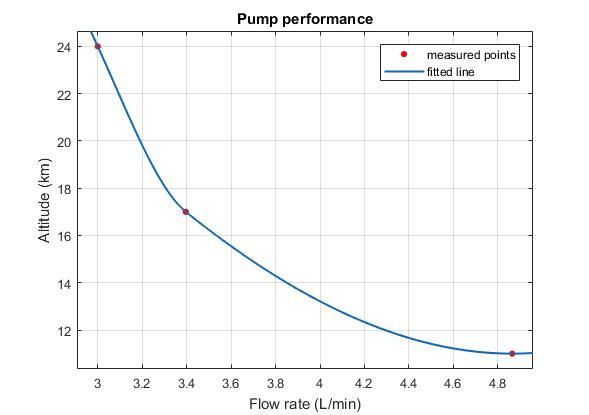
\includegraphics[width=11cm]{5-experiment-verification-and-testing/img/pump-performance.jpg}
    \end{align*}
    \caption {Obtained Pump Performance at Low Pressure.} \label{fig:pump-performance}
\end{figure}

\subsubsection{Test 30: Sampling Bag Bursting}
\label{sec:test30result}

A sampling bag was placed in a small vacuum chamber connected to the pump with the same set up as in Test 18, see Figures \ref{fig:pump-low-pressure-set-up} and \ref{fig:pump-low-pressure-progress}. The pump was run for 3 minutes with a full bag to see how the bag reacted. No changes were observed in the bag and no leaks appeared whilst it was in the testing chamber. Upon returning it to atmospheric levels it also appeared to be able to withstand the over pressure. The bag was then left, with the valve closed, on a table where it was handled a little during this time. Approximately 30 minutes after the test the bag made an audible popping noise and air leaked out. The damage that occurred to the bag during the burst can be seen in Figure \ref{fig:bag-burst-front} for the front of the bag and Figure \ref{fig:bag-burst-back} for the back of the bag.

\begin{figure}[H]
    \begin{align*}
        \includegraphics[width=1\linewidth]{5-experiment-verification-and-testing/img/bag-burst-front.png}
    \end{align*}
    \caption {Photo Showing the Extent of Damage on the Front of the Bag Due to Bursting.} \label{fig:bag-burst-front}
\end{figure}

\begin{figure}[H]
    \begin{align*}
        \includegraphics[width=1\linewidth]{5-experiment-verification-and-testing/img/bag-burst-back.png}
    \end{align*}
    \caption {Photo Showing the Extent of Damage on the Back of the Bag Due to Bursting.} \label{fig:bag-burst-back}
\end{figure}

This kind of bag failure could occur if bags are overfilled, particularly during ascent.

Next the system was set-up in the same way with a new bag. This time the pump was continuously run until failure occurred. This took around 6 minutes. The bag failed along the lower seam close to the valve and also at the valve connection. At the valve connection the bag ripped just above the valve. This time the burst was more energetic with the bottom of the bag moving outwards. Upon inspection the bottom of the bag was completely open and the part of the bag connected to the valve partially ripped open. In addition at the top of the bag small failures similar to those seen in Figure \ref{fig:bag-burst-front} were seen again. It is therefore thought that the bag was starting to fail at both the top and the bottom of the bag and but the bottom failed first.

The damage can be seen in Figures \ref{fig:seam-break} and \ref{fig:valve-rip}. It should be noted that the white bag valve was pulled off after the test and before photos were taken.

\begin{figure}[H]
    \begin{align*}
        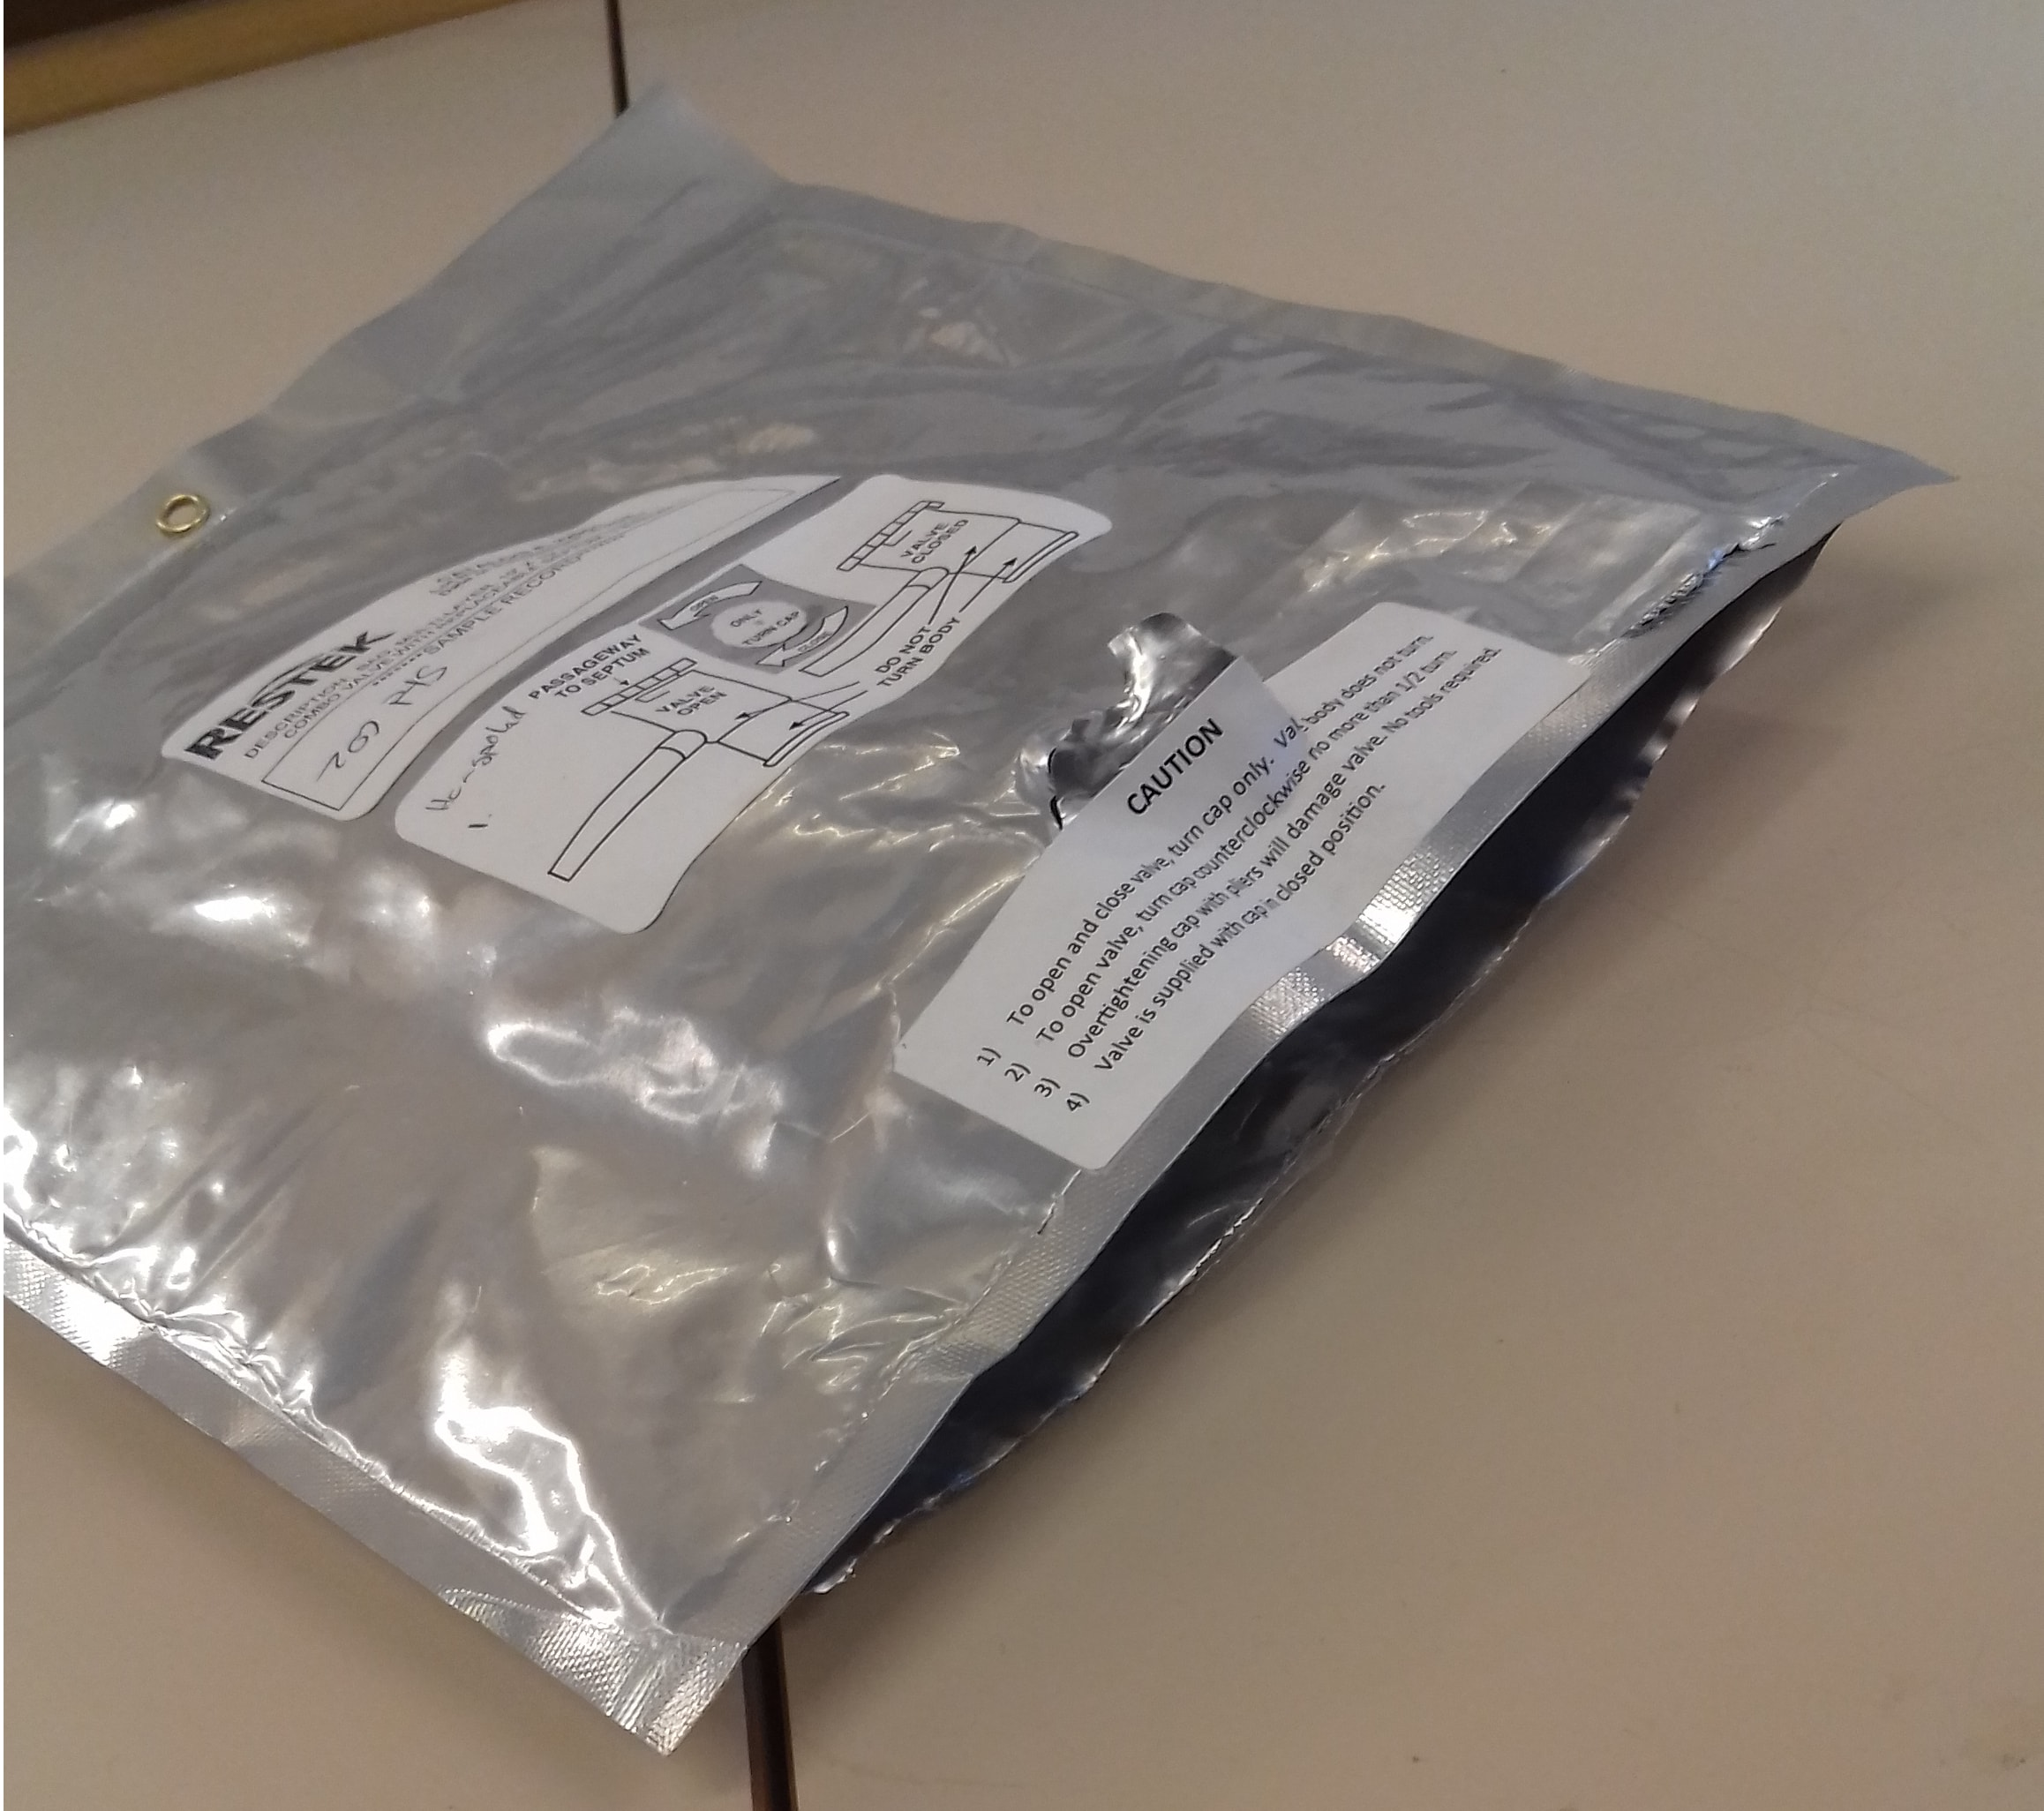
\includegraphics[width=1\linewidth]{5-experiment-verification-and-testing/img/bag-seam-break.jpg}
    \end{align*}
    \caption {Photo Showing the Damage Sustained to the Bottom of the Bag After Bursting Due to Continuous Pumping.} \label{fig:seam-break}
\end{figure}

\begin{figure}[H]
    \begin{align*}
        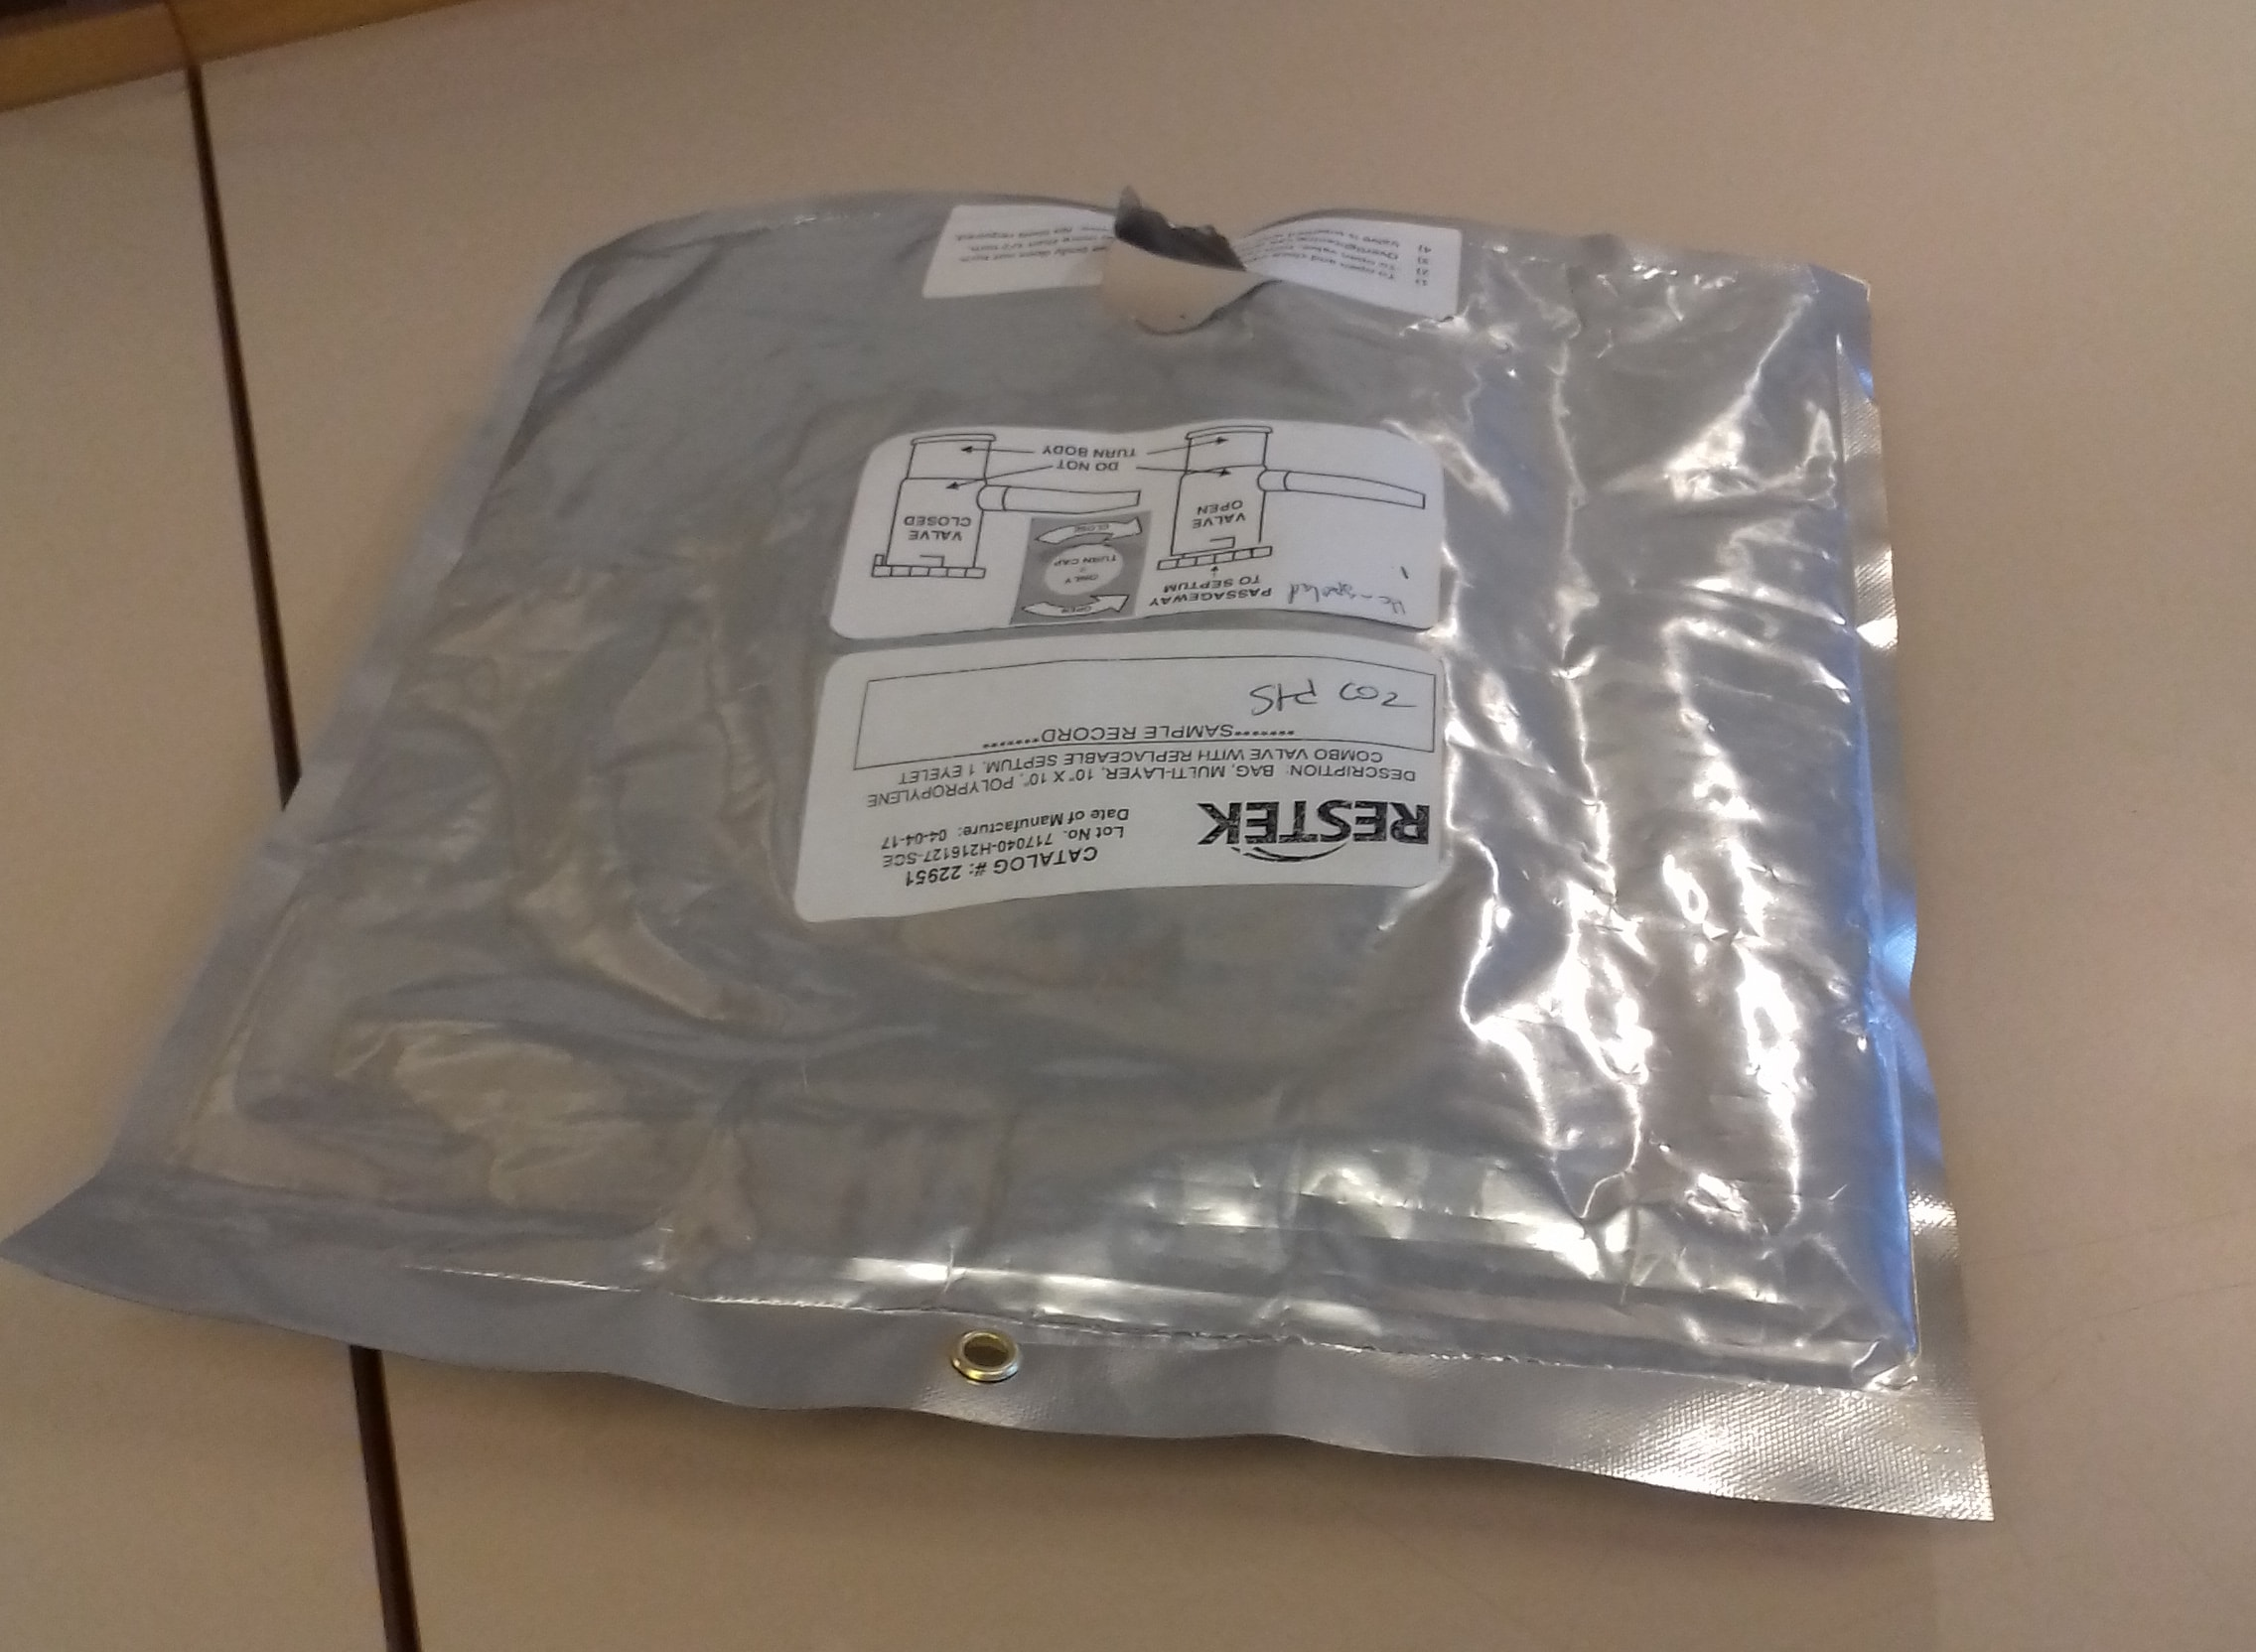
\includegraphics[width=1\linewidth]{5-experiment-verification-and-testing/img/bag-valve-break.jpg}
    \end{align*}
    \caption {Photo Showing Where the Bag Ripped Around the Valve.} \label{fig:valve-rip}
\end{figure}

This kind of bag failure could occur if there is a software error that results in the pump not switching off or a valve not closing, or if there is a malfunction in one of the valves which means it fails to close.

From the damage seen on the bags and from witnessing the burst it can be concluded that, as long as the bags are well secured to the valves at the bottom and through the metal ring at the top, bag bursting during flight would not cause damage to any other components on board. Even during the more energetic burst that occurs from continuous pumping the bag remained fixed to the valve connection and experienced no fragmentation. The consequences of a single bag burst would be limited to loss of data and a disturbance to audio frequencies. 

\subsection{Test 29: Pump Current under Low Pressure}
\label{sec:test29result}

This test was set up in the same way as above in Test 18, see Figure \ref{fig:pump-low-pressure-set-up} and \ref{fig:pump-low-pressure-progress}. The addition to this test was a multimeter to read the current that the pump was drawing. The pump was tested once with the outlet attached to a bag and once with the outlet sealed. This provides the current when the pump is pumping into an ambient pressure and into a higher pressure.

In general it was found for both cases that decreasing the pressure, or increasing the altitude, lead to a decrease in pump current draw. It was noted that there was an increase in current draw in between sea level conditions and 11 km altitude conditions. However as the lowest sampling point it intended to be at 11 km this should not be a problem for the experiment. The full results can be seen in Table \ref{tab:pumpcurrentpressure}. 

\begin{table}[H]
\centering

\begin{tabular}{|l|l|l|l|}
\hline
\textbf{Altitude (km)} & \textbf{Pressure (hPa)} & \textbf{Into Bag Current (mA)} & \textbf{Into Seal Current (mA)} \\ \hline
20 & 57 & 140 & 138 \\ \hline
18 & 68 & 150 & 141 \\ \hline
16 & 100 & 161 & 146 \\ \hline
12 & 190 & 185 & 175 \\ \hline
9 & 300 & - & 200 \\ \hline
6 & 500 & - & 242 \\ \hline
0 & 1013 & - & 218 \\ \hline
\end{tabular}
\caption{Table Showing How the Current Draw of the Pump Changed With Outside Air Pressure for Two Different Conditions. The First Pumping Into a Sampling Bag and the Second Pumping Into a Sealed Tube.}
\label{tab:pumpcurrentpressure}
\end{table}

A graphical representation of these results are shown in Figures \ref{fig:pumpcurpresbag} and \ref{fig:pumpcurpres}. From the table and figures it can be seen that the current draw is higher during the bag filling than during the sealed case. As the experiment will sample between 11 km and 24 km it can be concluded that the highest current draw will occur during the 11 km altitude sample and can be expected to be around 200 mA. 

\begin{figure}[H]
    \begin{align*}
        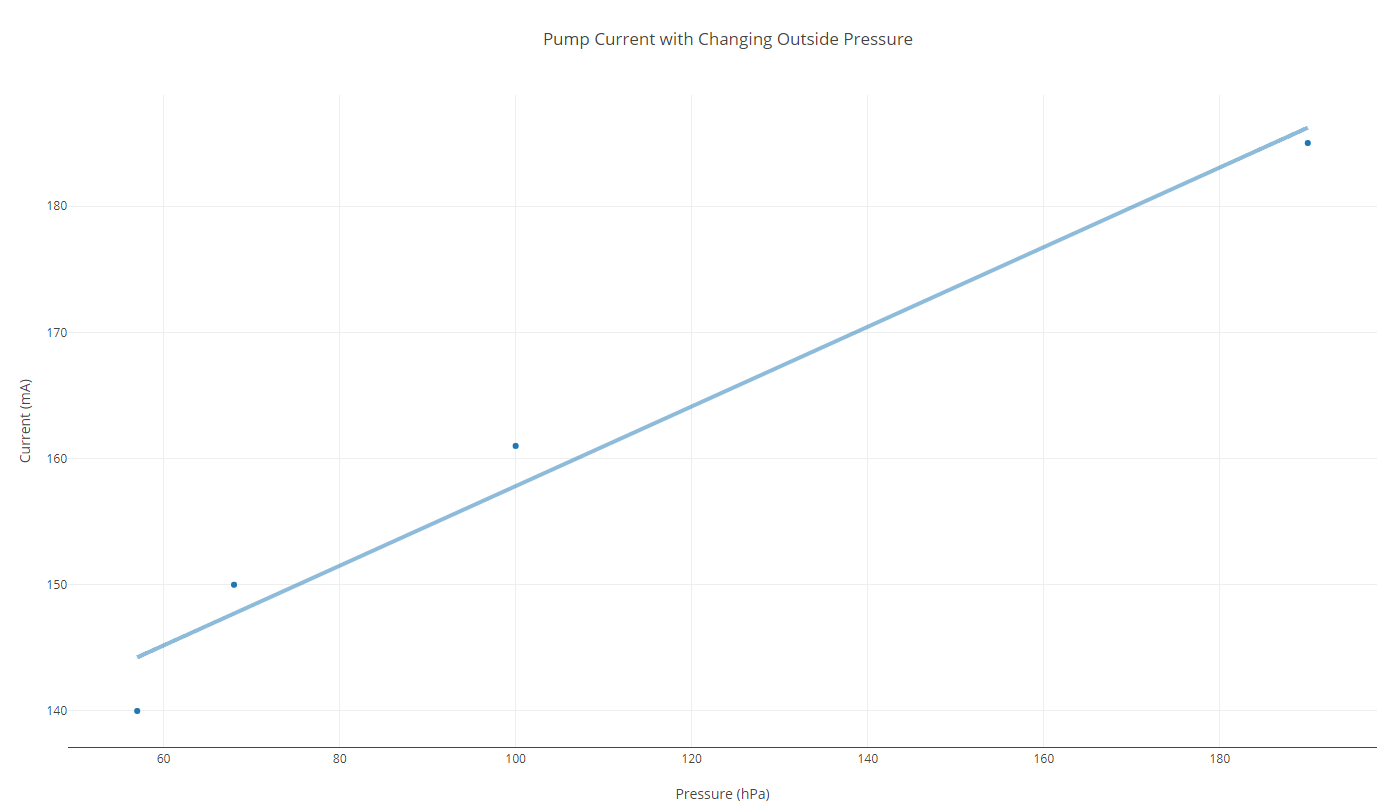
\includegraphics[width=1\linewidth]{5-experiment-verification-and-testing/img/pump-cureent-pressure.png}
    \end{align*}
    \caption {Graph Showing the Expected Current Values When the Pump is Pumping Air Into a Bag Based Upon the Results Obtained.} \label{fig:pumpcurpresbag}
\end{figure}


\begin{figure}[H]
    \begin{align*}
        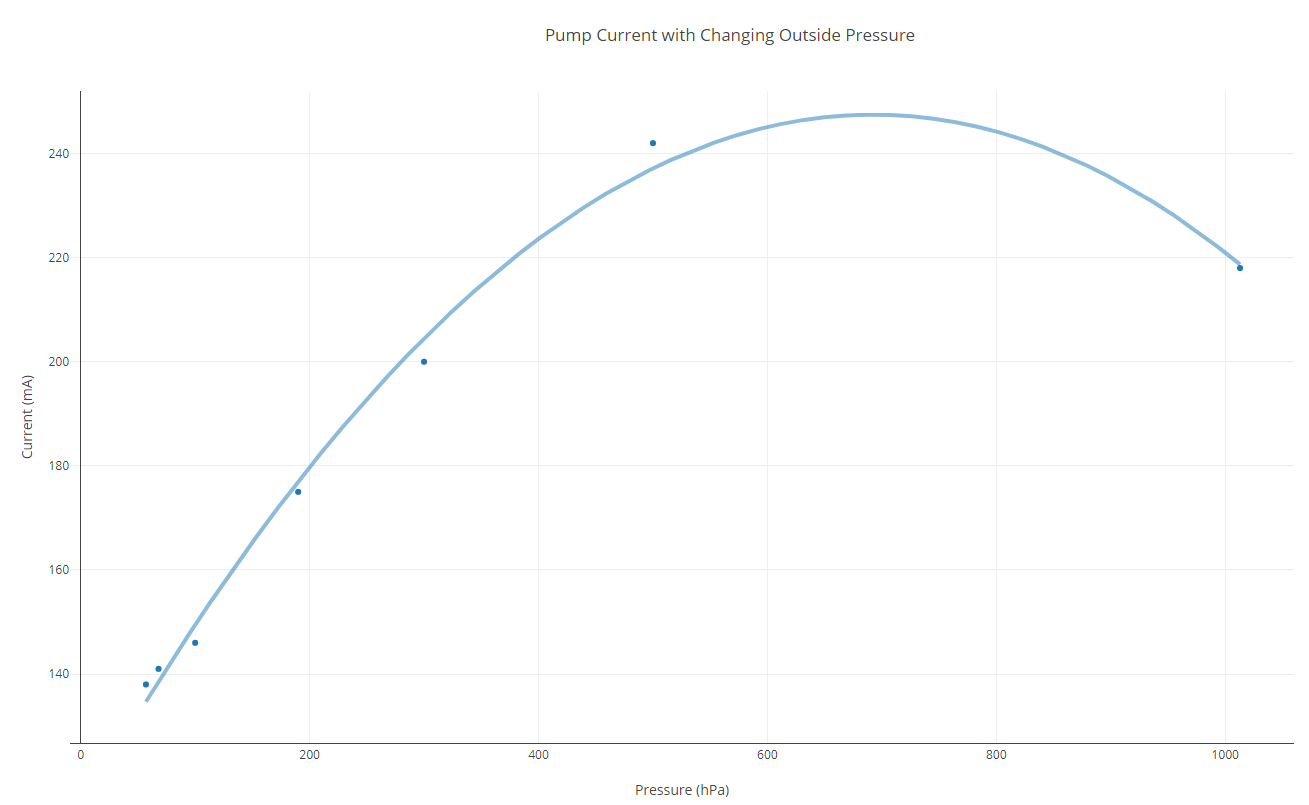
\includegraphics[width=1\linewidth]{5-experiment-verification-and-testing/img/pump-current-pressure.png}
    \end{align*}
    \caption {Graph Showing the Expected Current Values When the Pump is Pumping Air Into a Sealed Outlet Based Upon the Results Obtained and the Data Shown In Figure \ref{fig:pumpflowcur}.} \label{fig:pumpcurpres}
\end{figure}

By looking at the data from both Test 18 and Test 29 a relationship can be seen between the outside air pressure, the flow rate of the pump and the current draw of the pump. 

\subsection{Test 17: Sampling bags' holding times and samples' condensation verification}
\label{sec:test17result}

The main objective of this test was to flush eight 1 L sampling bags with nitrogen, the same way it will be done for the flight. After the flushing is done, fill them with a dry gas and leave them outside for 6, 14, 24 and 48 hours. Then analyze two sampling bags after each time duration and see if the concentration of gases inside has changed. 

A dry gas is a gas of high concentration of $CO$ and low $H_2O$ and its exact concentration can be known by comparison to the calibrating gas in the Picarro analyzer. Therefore, the concentration when sampling the bags is known and it can be compared with the concentration after analysis. If the sampling bags can hold the samples for 48 hours then when analyzing, the concentration of gases should not change. If condensation occurs that will be seen as an increase in water vapour concentration. 

Note that the size of the sampling bags was not the same as the size that will be used during the experiment. The reasons were availability of 1 L sampling bags at FMI and a first assumption that the size would not affect the results. The sampling bags were exactly the same model/material.


This test was realized at FMI in Sodankyl\"{a}. Eight Multi-Layer Foil bags of 1 L volume were connected to SMC valves as shown in Figure \ref{fig:bag-valve-quick-connector} and all together connected in series with stainless steel tubes as can be seen in Figure \ref{fig:bags-test-set-up}.

\begin{figure}[H]
    \begin{align*}
        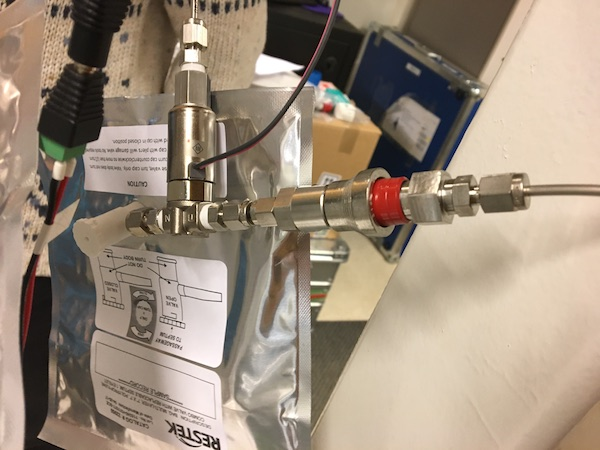
\includegraphics[width=1\linewidth]{5-experiment-verification-and-testing/img/bag-valve-quick-connector.jpg}
    \end{align*}
    \caption {1 L Sampling Bag With SMC Valve Attached to It. The Valve is at One of the Ends of the System so a Quick Connector is Connecting it to the Tube That Goes to the Nitrogen Bottle/Vacuum Pump.} \label{fig:bag-valve-quick-connector}
\end{figure}


\begin{figure}[H]
    \begin{align*}
        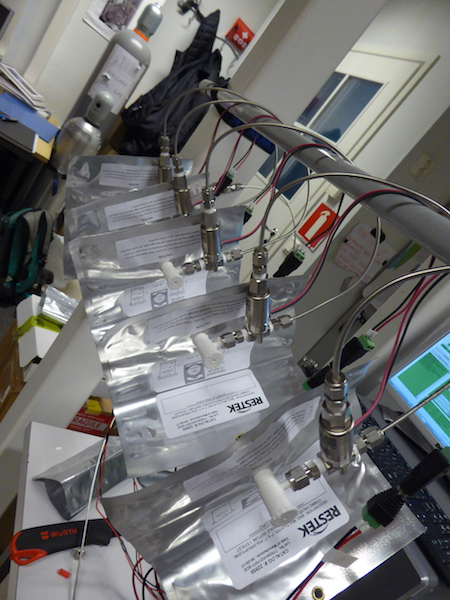
\includegraphics[width=1\linewidth]{5-experiment-verification-and-testing/img/bags-test-set-up.jpg}
    \end{align*}
    \caption {Sampling Bags System Connected in Series.} \label{fig:bags-test-set-up}
\end{figure}

Figure \ref{fig:bags-test-general-overview} shows a general overview of the experiment set up before the sampling bags were attached to the SMC valves. The picture shows the eight SMC valves hanging on a bar and red and black cables connecting them to the switches. It can also be seen a nitrogen bottle standing at the right side of the table and a vacuum pump under the table. Figure \ref{fig:nitrogen-vacuum-valve} shows the pressure sensor on the table, a flow-metre, a needle valve that adjusts the flow rate and a valve. This valve was used to control the filling and flushing of the sampling bags realized with nitrogen. The position shown in Figure \ref{fig:nitrogen-vacuum-valve} is for vacuuming, the pump is sucking the air from the sampling bags and the nitrogen tube is closed. The valve position for filling is the opposite, opening the nitrogen tube and closing the vacuum. There is also an intermediate position that closes both, nitrogen and vacuum. 



\begin{figure}[H]
    \begin{align*}
        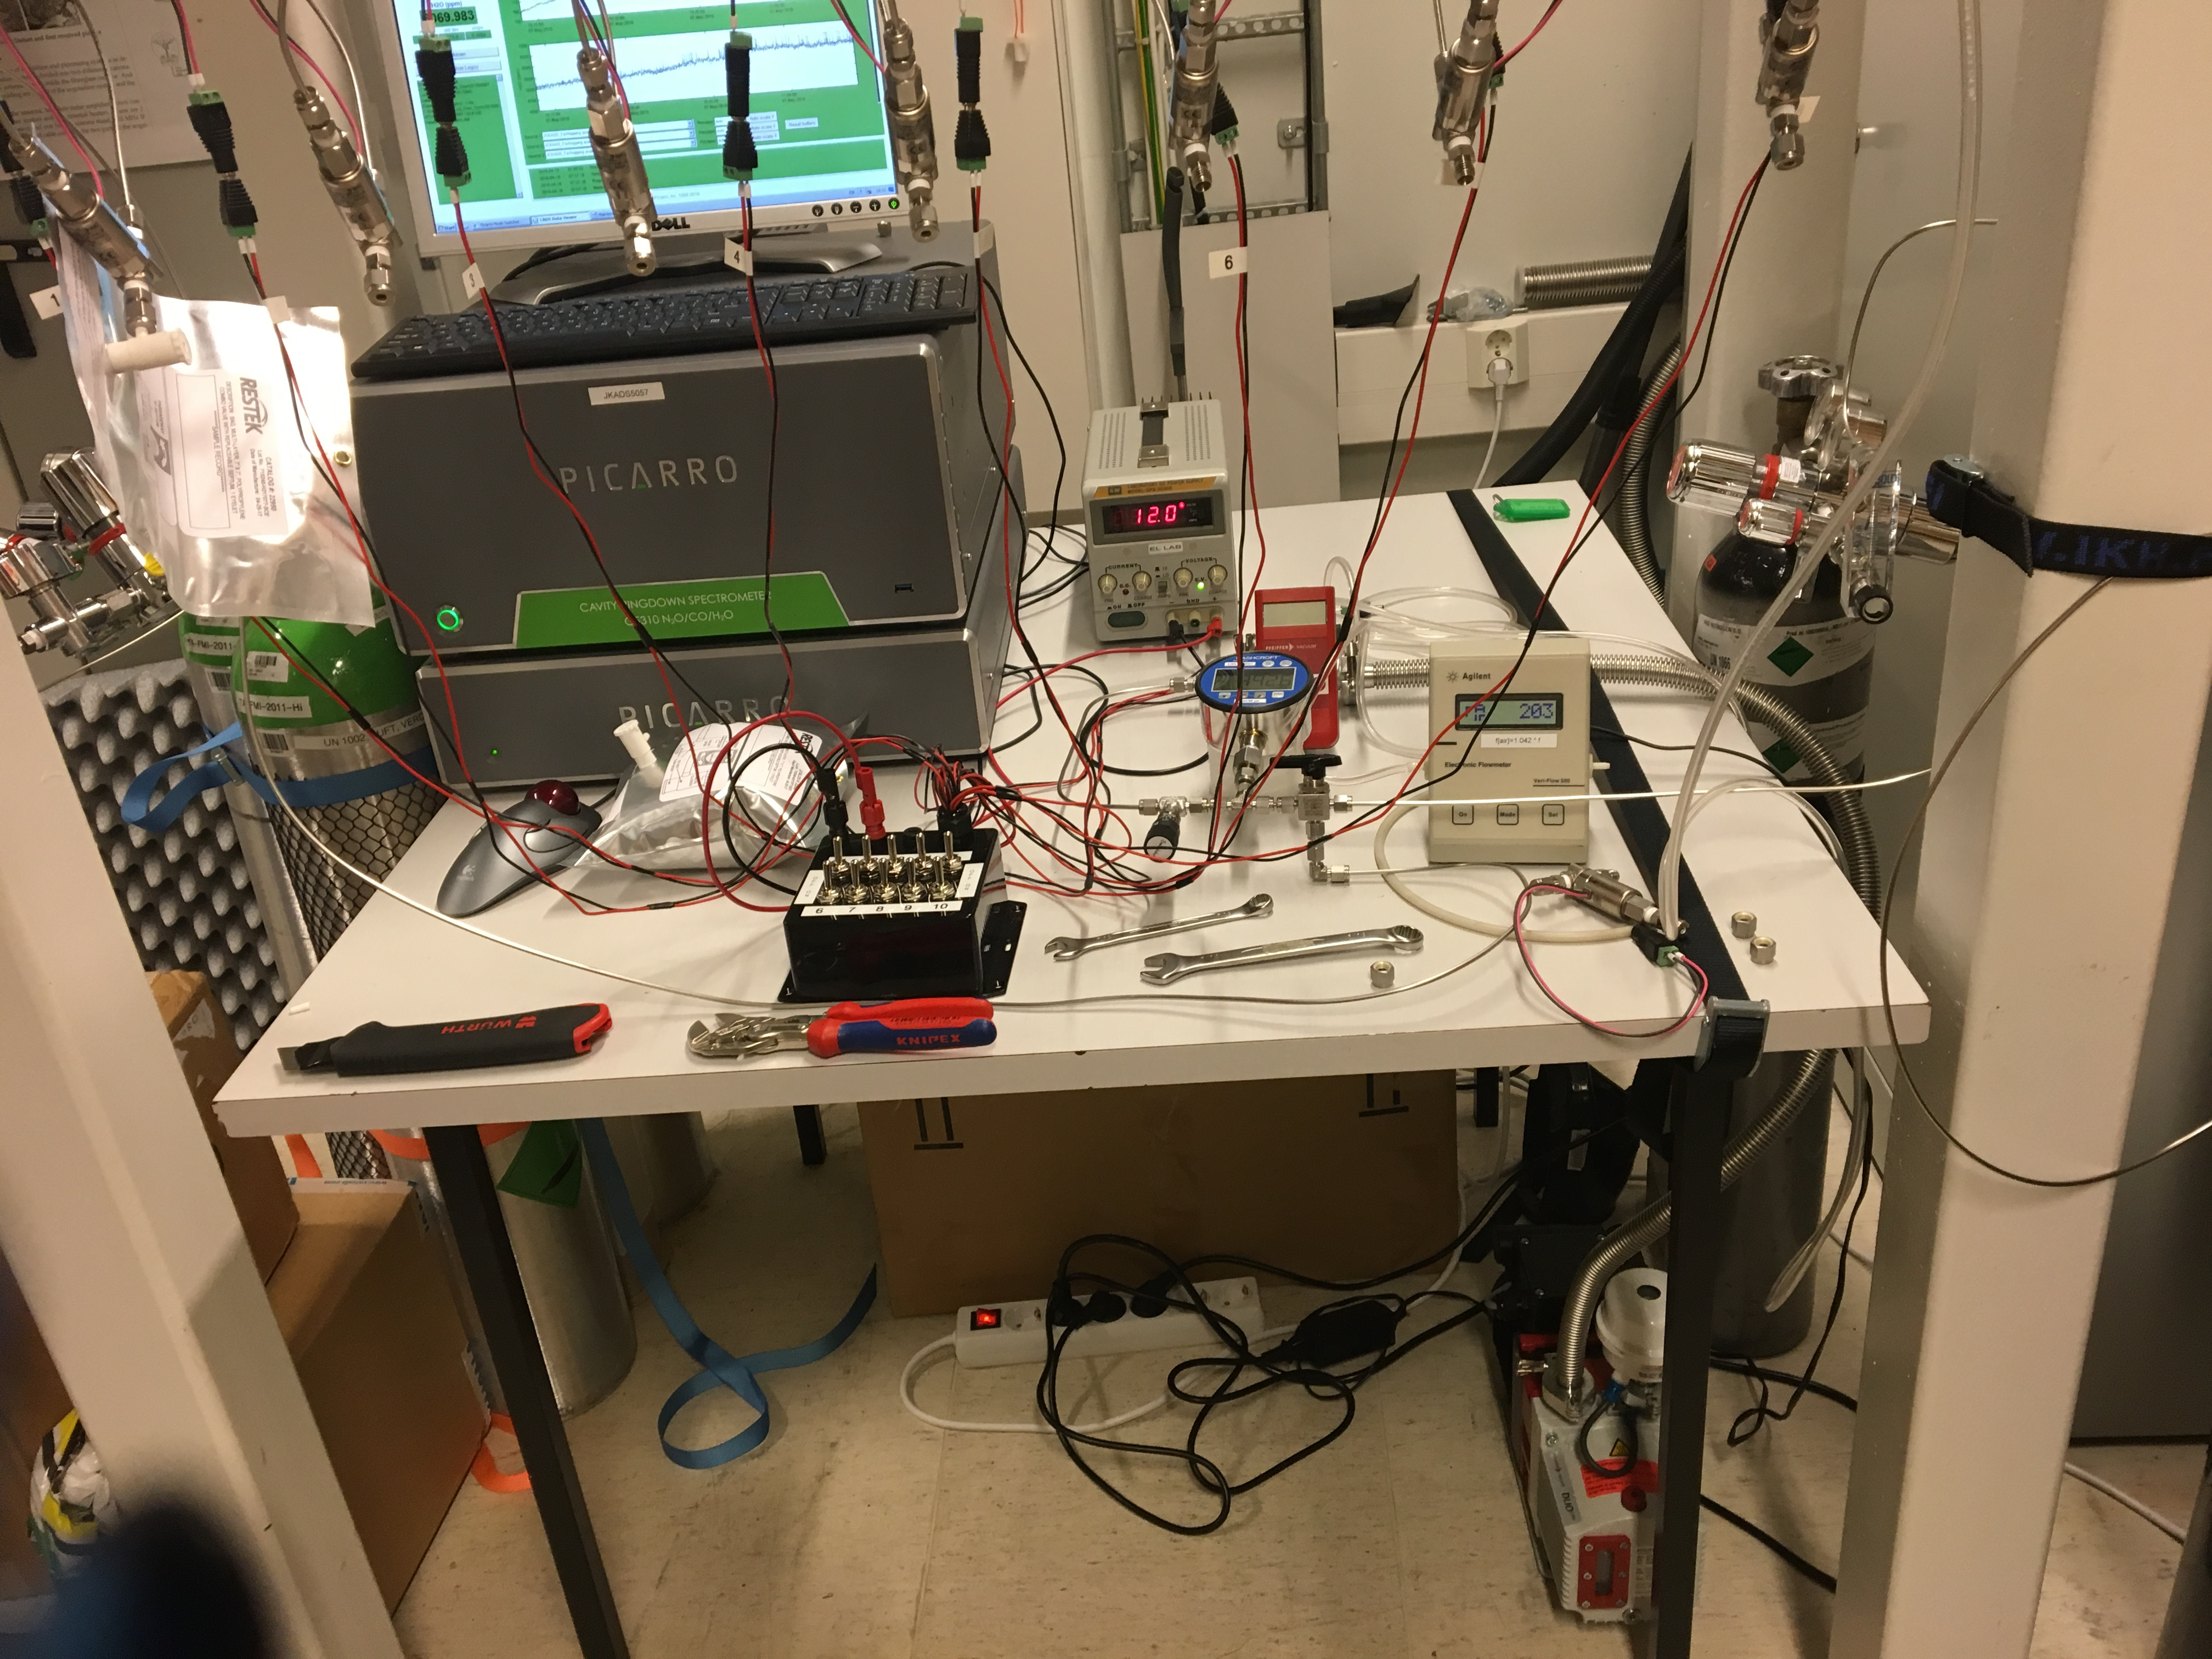
\includegraphics[width=1\linewidth]{5-experiment-verification-and-testing/img/bags-test-general-overview.jpg}
    \end{align*}
    \caption {General Overview of the test Set up Before the Sampling Bags Were Attached to the Valves} \label{fig:bags-test-general-overview}
\end{figure}



\begin{figure}[H]
    \begin{align*}
        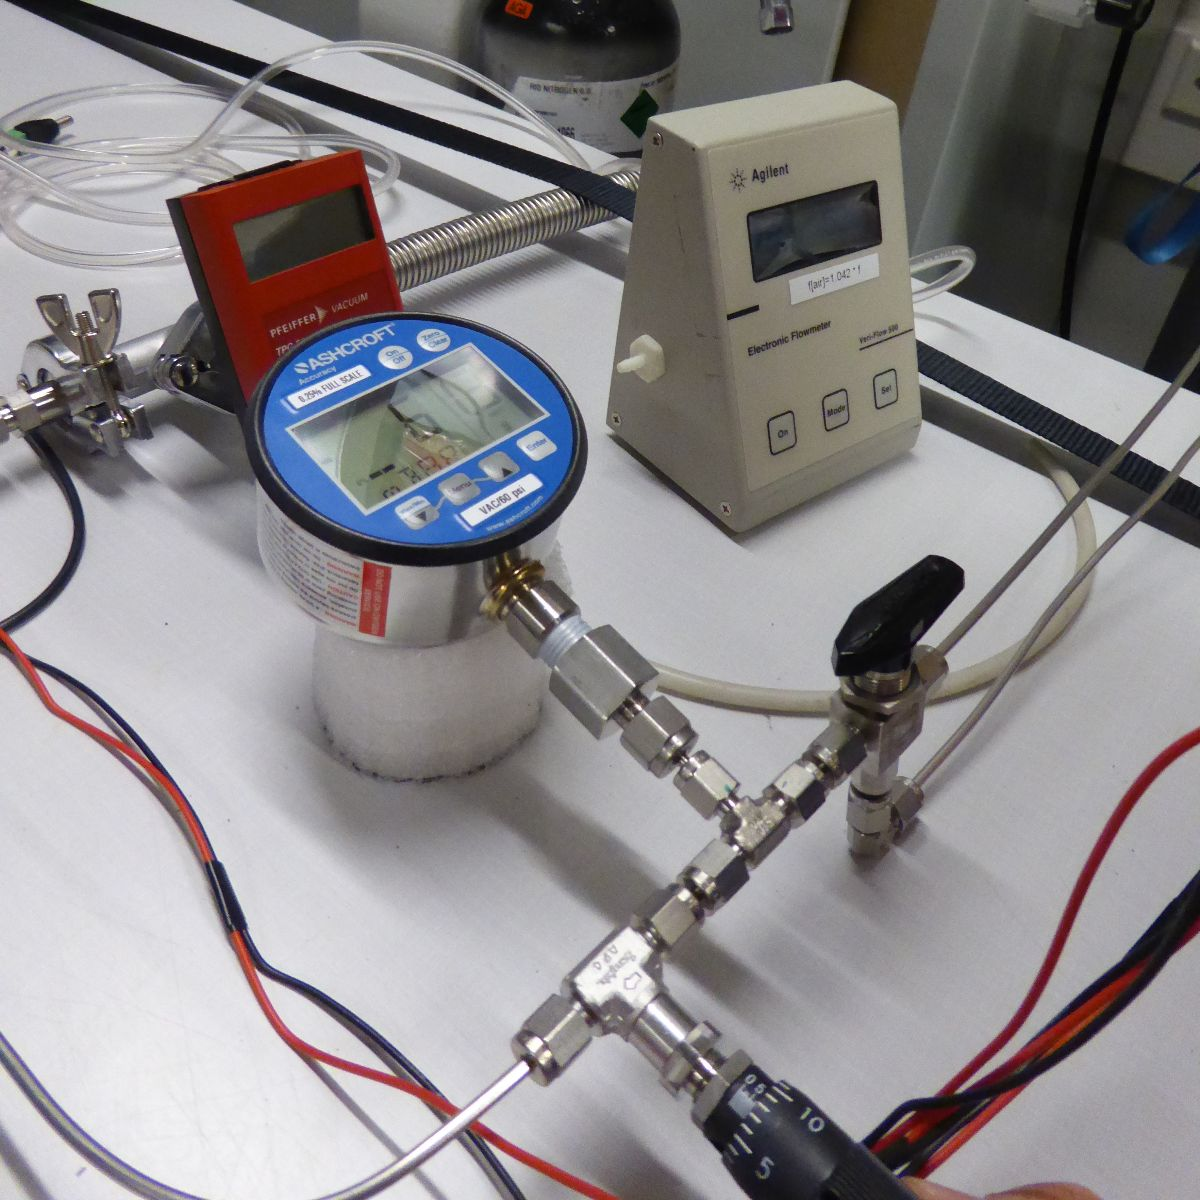
\includegraphics[width=1\linewidth]{5-experiment-verification-and-testing/img/nitrogen-vacuum-valve.jpg}
    \end{align*}
    \caption {Valve that Controls Filling/Vacuum in of the Sampling Bags. Pressure Sensor, Flow-metre and Needle Valve.} \label{fig:nitrogen-vacuum-valve}
\end{figure}


The procedure during the test was as follows: 
\begin{itemize}
    \item Set up all the connections between pump, nitrogen bottle, valves system in series. 
    \item Attach the sampling bags to the SMC valves. 
    \item Start flushing the tubes with nitrogen. For this all the sampling bags' valves are closed. 
    \item Adjust the flow rate of nitrogen at 500 ml/min. 
    \item Open sampling bags' manual valves (not to be confused with the SMC valves which are still all closed).
    \item Turn on valve 1. Fill sampling bag number 1 for 2 minutes. Turn off valve 1. Repeat it for the seven sampling bags left.  
    \item Change the valve seen in Figure \ref{fig:nitrogen-vacuum-valve} to vacuum position and empty the bags.
    \item Flush the tubes after all the sampling bags have been emptied. This is to remove as much air as possible that could be left inside the sampling bags.
    \item Repeat the flushing for two more times. 
    \item Change the nitrogen bottle for the dry gas bottle. 
    \item Flush the tubes with nitrogen. 
    \item Fill the eight sampling bags one by one. 
    \item Take the sampling bags outside as shown in Figure \ref{fig:bags-outside} to simulate the conditions at which they will be exposed after landing. 
\end{itemize}

\begin{figure}[H]
    \begin{align*}
        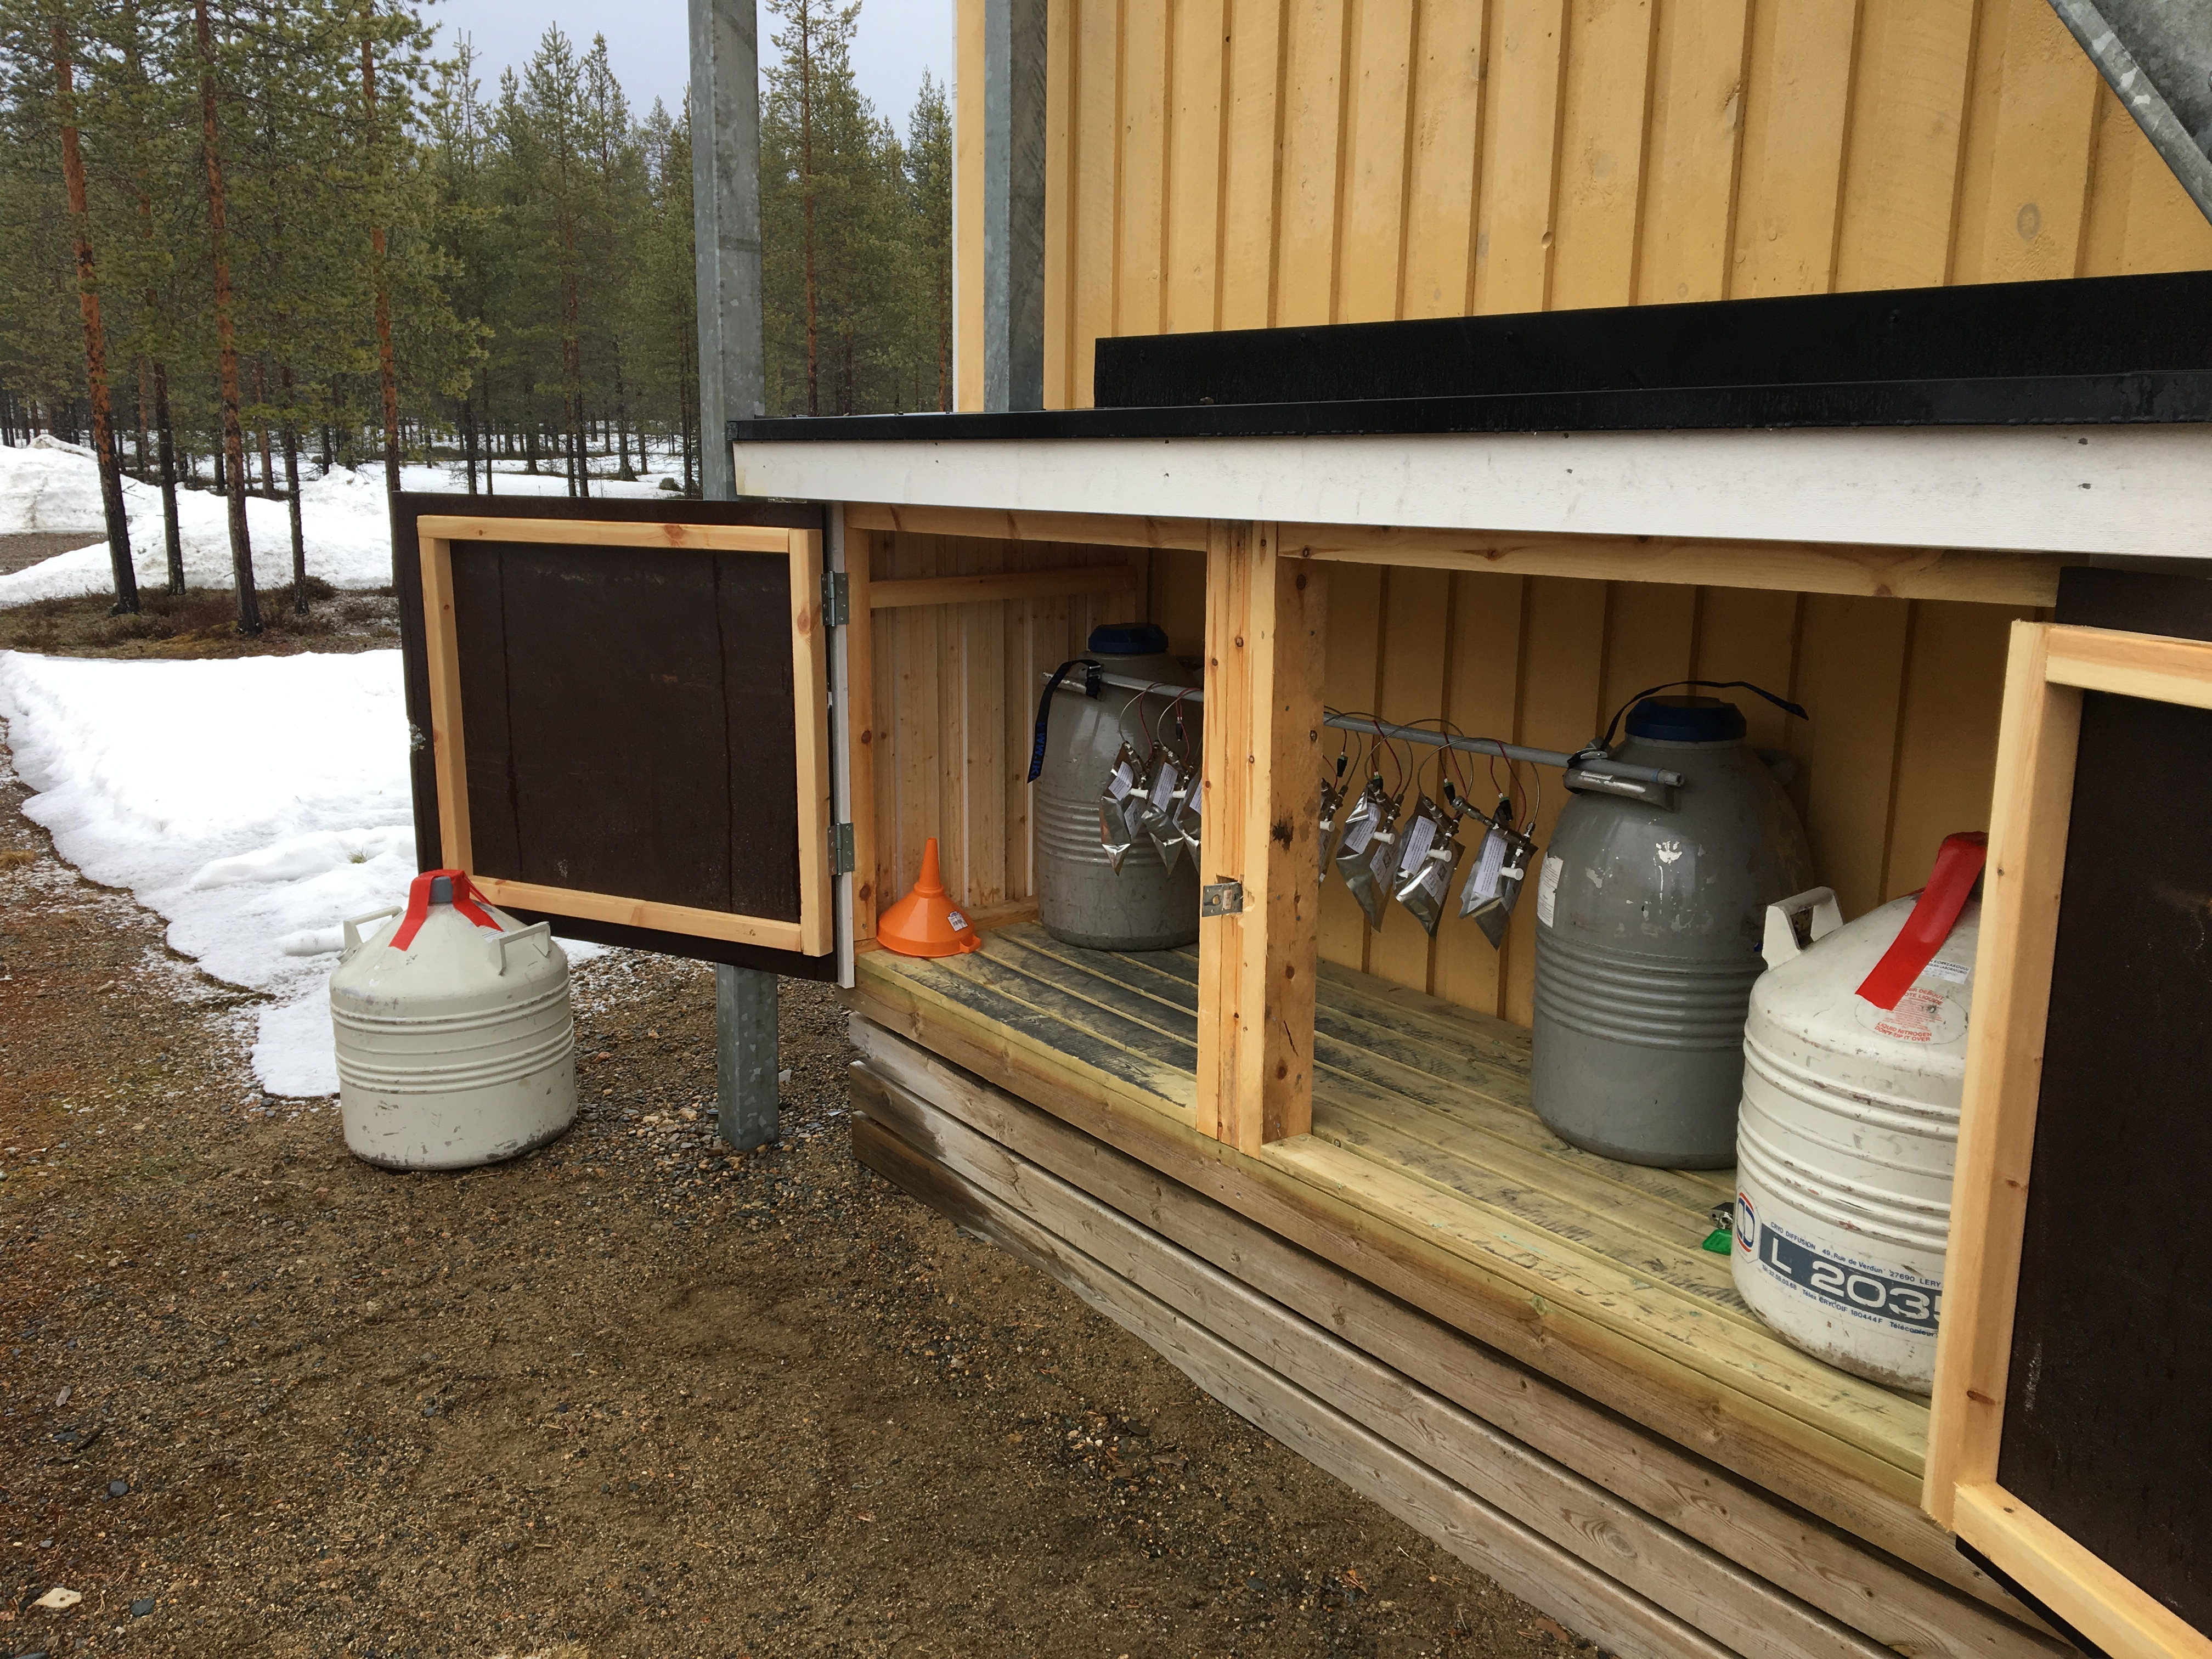
\includegraphics[width=1\linewidth]{5-experiment-verification-and-testing/img/bags-outside.jpg}
    \end{align*}
    \caption {Sampling Bags Left Outside Waiting to be Analyzed.} \label{fig:bags-outside}
\end{figure}

After each of the mentioned times, 6, 14, 24 and 48 hours, two sampling bags were taken inside the laboratory to be analyzed. The procedure to analyze was: 
\begin{itemize}
    \item Have the dry gas flowing through the Picarro analyzer for at least one hour before the analysis. This is to avoid having moisture inside the tubes and have stable measurements of concentrations.
    \item Flush the tubes in between the two sampling bags with dry gas. For that the dry gas has to be disconnected from the analyzer and moisture would get into the Picarro. To avoid this, calibrating gas is flowing through the analyzer while the tubes are being flushed.
    \item Connect the system formed by two sampling bags with one end to the dry gas bottle and the other to the Picarro inlet.
    \item Wait for one hour until the readings of dry gas concentrations are stable. 
    \item Open the valve of the first sampling bag. 
    \item Right after the first sampling bag is empty, close its valve and open the valve for the next one. 
    \item Keep the dry gas flowing for one more hour after analysis. 
\end{itemize}

After analyzing the sampling bags the obtained results are presented in Figure \ref{fig:test17-results}.

\begin{figure}[H]
    \begin{align*}
        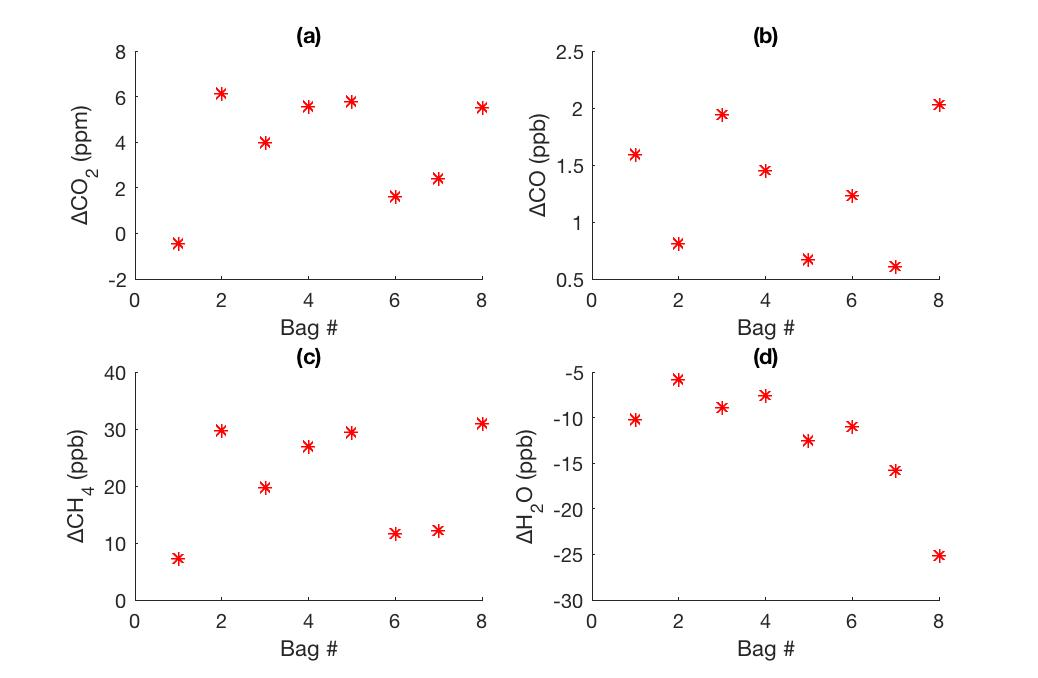
\includegraphics[width=1\linewidth]{5-experiment-verification-and-testing/img/test17-results.jpg}
    \end{align*}
    \caption {Obtained Variation in Concentration for (a) $CO_2$ in ppm, (b) $CO$ in ppb, (c) $CH_4$ in ppb and (d) $H_2O$ in ppb.} \label{fig:test17-results}
\end{figure}


It should be mentioned that the results were not at all what was expected. If the sampling bags held the gases for 48 hours, the analyzed concentration should have been the same as the dry gas used to fill them or the variation should have been smaller. 

A possible explanation for this results could be that the emptying of the sampling bags was not done rigorously enough and that some air/nitrogen was left inside which diluted in the dry gas and changed the concentrations. This effect is even increased due to the smaller size of the used sampling bags (1 L instead of 3 L). This would also explain why the results don't follow any pattern. 

The general outcome of this test is that the team has realized that the flushing of the sampling bags is a very delicate process. This test will be repeated but using the set-up described in Section 4. This test has also been useful to decide that the flushing of the sampling bags should be done with dry gas instead of nitrogen in order to minimize the effects of the nitrogen diluting in the samples. 

% Flushing with nitrogen may alter the results. 
